\documentclass[12pt,a4paper]{article}

% Essential packages
\usepackage[utf8]{inputenc}
\usepackage[T1]{fontenc}
\usepackage[english]{babel}
\usepackage{amsmath,amsfonts,amssymb}
\usepackage{graphicx}
\usepackage{hyperref}
\usepackage{geometry}

% Page geometry
\geometry{margin=1in}

% Hyperlink setup
\hypersetup{
    colorlinks=true,
    linkcolor=blue,
    filecolor=magenta,      
    urlcolor=cyan,
    citecolor=red
}

% Title page information
\title{AImpact: Your AI co-founder. Whitepaper}
\author{Denys Riabtsev, Kostiantyn Ostapenko \\ OSTOLEX \\ \texttt{denys@ostolex.com, kostiantyn@ostolex.com}}
\date{\today}

\begin{document}

% Title page
\maketitle

% Abstract
\begin{abstract}
AImpact represents an AI-powered platform designed to democratize Web3 development by enabling users to create blockchain applications through natural language prompts. It eliminates traditional coding barriers, allowing users to describe their Web3 project ideas in plain language and receive fully functional applications in return. The platform's AI-driven approach reduces development time and complexity while maintaining the security and functionality expected from Web3 applications. 
\end{abstract}

% Keywords (optional)
\noindent\textbf{Keywords:} artificial intelligence, Web3, blockchain, Solana, smart contracts, decentralized applications, AI-powered development, prompt-based programming, DApp generation

\newpage

% Table of contents
\tableofcontents
\newpage

% Main content
\section{Introduction}
\label{sec:introduction}

The rapid evolution of blockchain technology and Web3 applications has created unprecedented opportunities for innovation in decentralized systems. However, the technical complexity of blockchain development remains a significant barrier to entry for many potential innovators. Traditional Web3 development requires extensive knowledge of specialized programming languages, blockchain protocols, and cryptographic principles, often deterring creative individuals and businesses from participating in this transformative technology.

AImpact emerges as a solution to this challenge by leveraging artificial intelligence to bridge the gap between ideas and implementation. Our platform transforms natural language descriptions into fully functional Web3 applications, democratizing access to blockchain technology and enabling a new wave of innovation in the decentralized space.

This whitepaper outlines the technical architecture, capabilities, and potential applications of AImpact.

\section{Userflow}
\label{sec:userflow}

The typical user flow for the AImpact platform consists of the following steps:

\begin{enumerate}
    \item \textbf{Project Description}: Users provide a natural language description of their desired Web3 application, including functionality, features, and requirements.
    
    \item \textbf{Application Design Generation}: The platform's AI system generates a user interface for the application. 
    User can continiously modify the design of the application with text prompts or images.
    
    \textit{Note: user can choose to skip this step and start developing frontend code without a design. 
    This is useful for quick prototyping and allow user to make changes to the design more easily.}
   
    \item \textbf{Frontend Code Generation}: 
    Based on the provided design, the AI generates the frontend code for the application. 
    Frontend is launched in a sandbox environment, where user can test the application and modify the code either with text prompts or with a visual code editor.
   
    \textit{Note: user can choose to skip this step and start developing smart contract code without a frontend component. }

    \item \textbf{Smart Contract Code Generation}: 
    Using provided description, the AI generates the smart contract code for the application. Under the hood, the AI uses a database with default smart contracts, MCP module and LLM for fine-tuning the code for the specific application (we will discuss this in more detail in the upcoming sections).
    Smart contract is also launched in a sandbox environment using locally run blockchain environment, where user can test the application and modify the code either with text prompts or with a visual code editor.
    

    \item \textbf{Testing}: 
    Having frontend and smartcontract launched locally in the sandbox environment, user tests the application.
    User can also test the application in the live environment, where the smartcontract is deployed to the chosen blockchain Testnet or Devnet (frontend is still running locally in the sandbox environment).
    

    \item \textbf{AI-based auditing}: 
    User can request an AI-based auditing of the smartcontract code.
    The AI audits the smartcontract code (using several LLMs) for security vulnerabilities and performance issues.
    System will provide a report with the results of the audit.
    User can request a fix for the issues found in the audit if any.
    
    
    \item \textbf{Deployment}: 
    When user is satisfied with the application, it can be deployed to production environment.

\end{enumerate}

\textbf{Limitations:}
\begin{itemize}
    \item User must connect their wallet in order to use the platform.
    \item User can only deploy the application to the chain that is supported by the wallet (for example, if user connected Solana wallet, they can only deploy the application to Solana blockchain).
    \item In order to use the platform user should purchase messages using their wallet.
    \item Fronted is deployed to the supported hosting provider, which is chosen by the platform. If user wants to deploy it elsewhere, they can do so by using the provided code.

\end{itemize}


\section{Technical Overview}
\label{sec:literature}


\subsection{AImpact Smart Contract Templates}

In order to improve generation of the smart contract code, the AImpact platform uses a database of smart contract templates. Those templates are 
selected by AImpact MCP module (we will discuss this in more detail in the upcoming sections).
LLM uses the selected template as a base for the smart contract code generation and fine-tunes it to the specific application.


\begin{figure}[h]
    \centering
    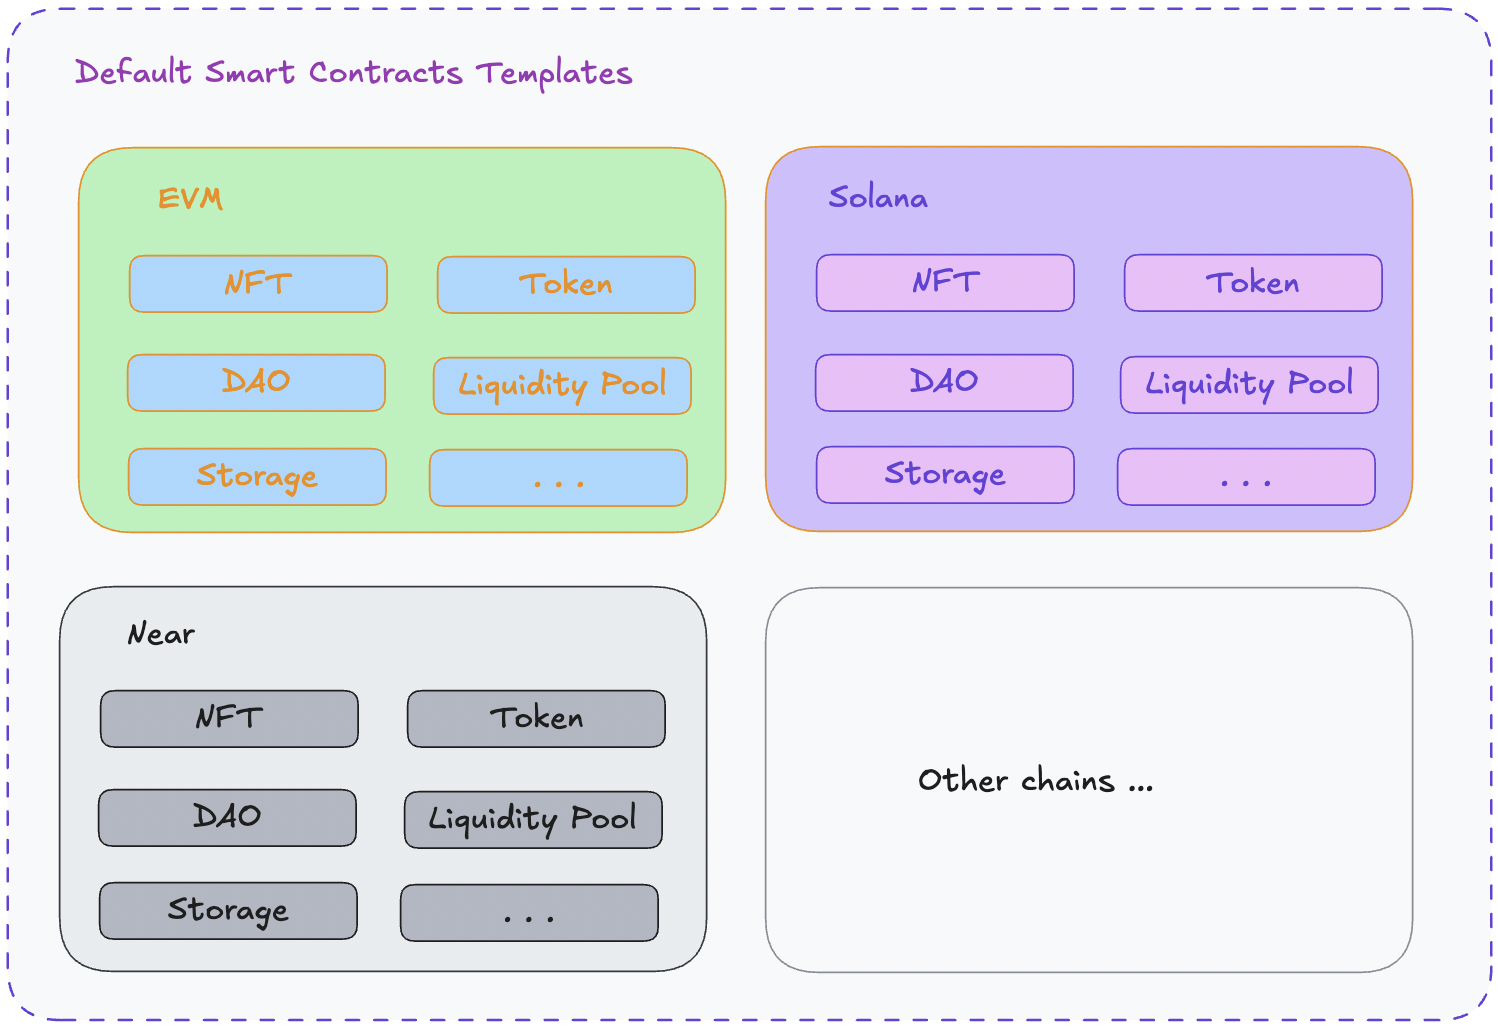
\includegraphics[width=0.7\textwidth]{imgs/templates.png}
    \caption{Smart contract templates}
    \label{fig:templates}
\end{figure}


\subsection{AImpact MCP Module}

The platform uses AImpact MCP module to interact with the smart contract code generation and deployment. It provides LLM a set of tools to
access the database of smart contract templates, deploy the smart contract either to the sandbox environment or to the chosen blockchain Testnet, 
Devnet or Mainnet, test the smart contract, deploy the frontend to the hosting provider.

\begin{figure}[h]
    \centering
    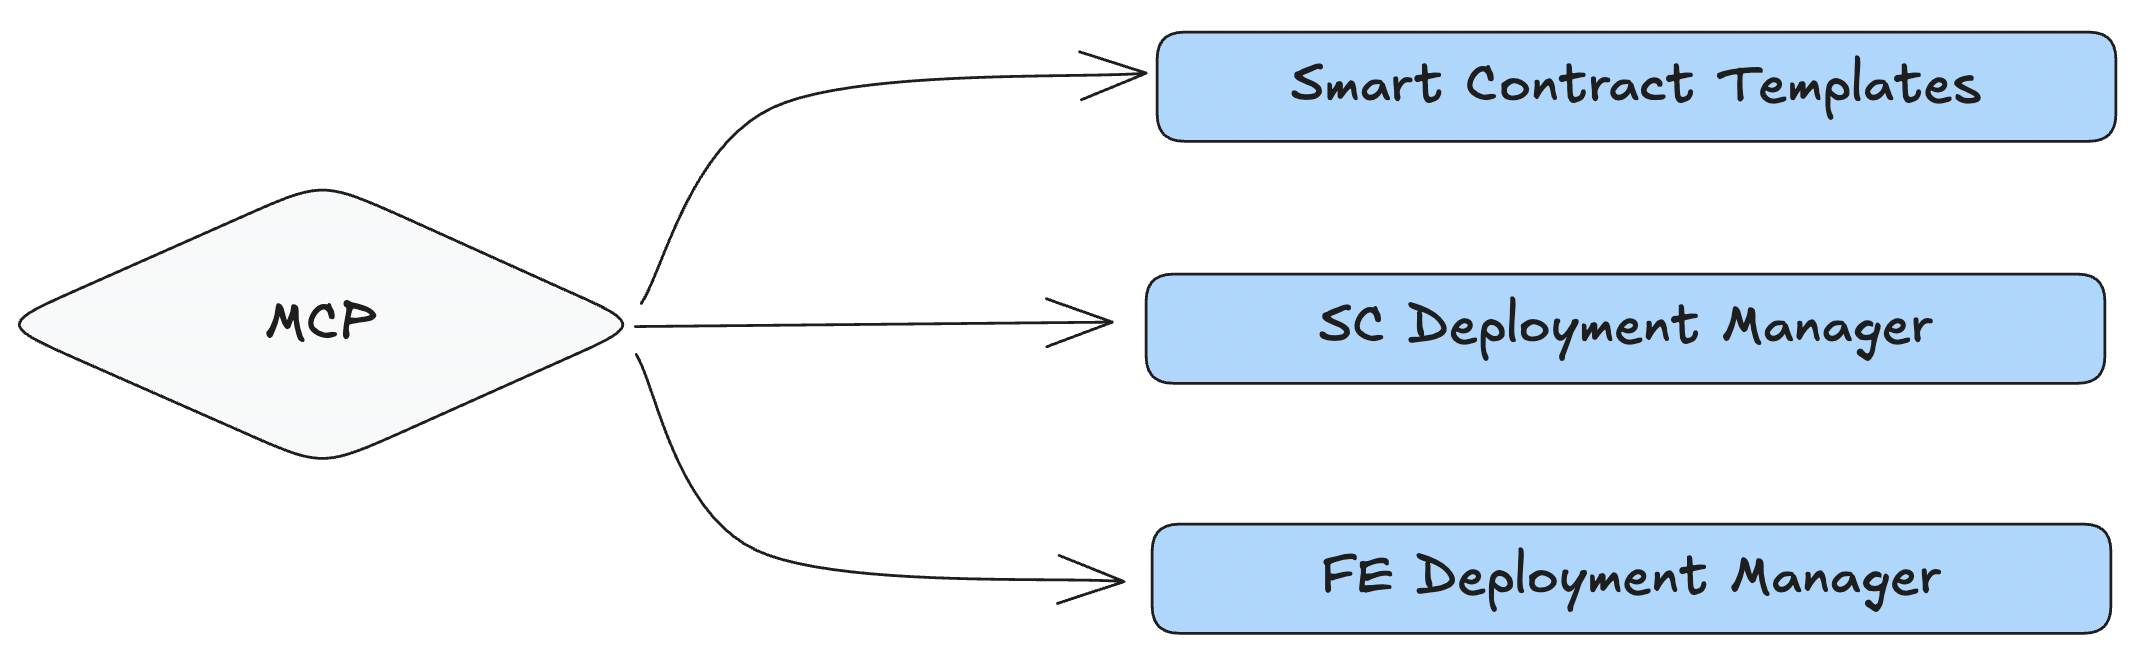
\includegraphics[width=0.7\textwidth]{imgs/mcp.png}
    \caption{AImpact MCP Module}
    \label{fig:mcp}
\end{figure}


\subsection{Deployment}

Deployment stages for the smart contract:
\begin{enumerate}
    \item \textbf{Sandbox Environment}: Locally run blockchain environment simulation of the chosen blockchain. 
    As it is an isolated environment, contract must be deployed on further stages in order to be accessible by other users.
    \item \textbf{Testnet / Devnet}: Deploy the smart contract to the chosen blockchain Testnet or Devnet. 
    AImpact also provides in-built tool for token airdrop request for project deployment.
    \item \textbf{Mainnet}: Production deployment of the smart contract.
\end{enumerate}

\begin{figure}[h]
    \centering
    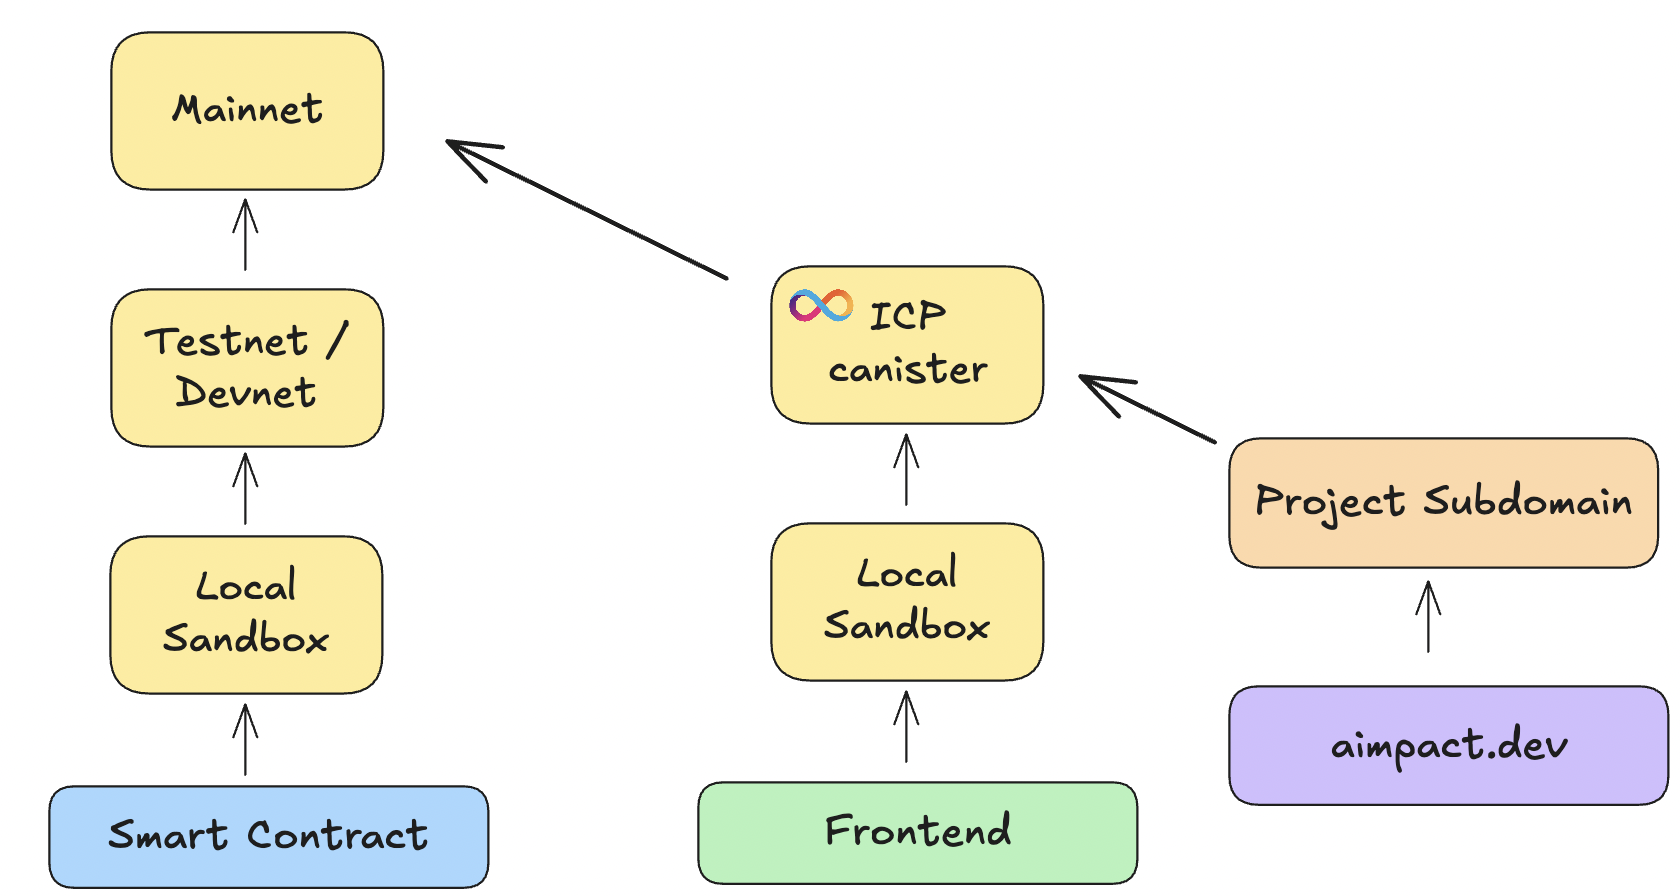
\includegraphics[width=0.7\textwidth]{imgs/deployment.png}
    \caption{Deployment of the Projects}
    \label{fig:deployment}
\end{figure}


Deployment stages for the frontend:
\begin{enumerate}
    \item \textbf{Sandbox Environment}: Locally run frontend environment simulation of the chosen hosting provider.
    Frontend can access the smart contract deployed in the sandbox environment.
    \item \textbf{Production Environment}: Deploy the frontend to the ICP canister.
\end{enumerate}

\textit{Note: AImpact provides subdomain for the frontend deployment which can be used to access the deployed frontend.}




\subsection{Scheme of AImpact Infrastructure Architecture}


\begin{figure}[h]
    \centering
    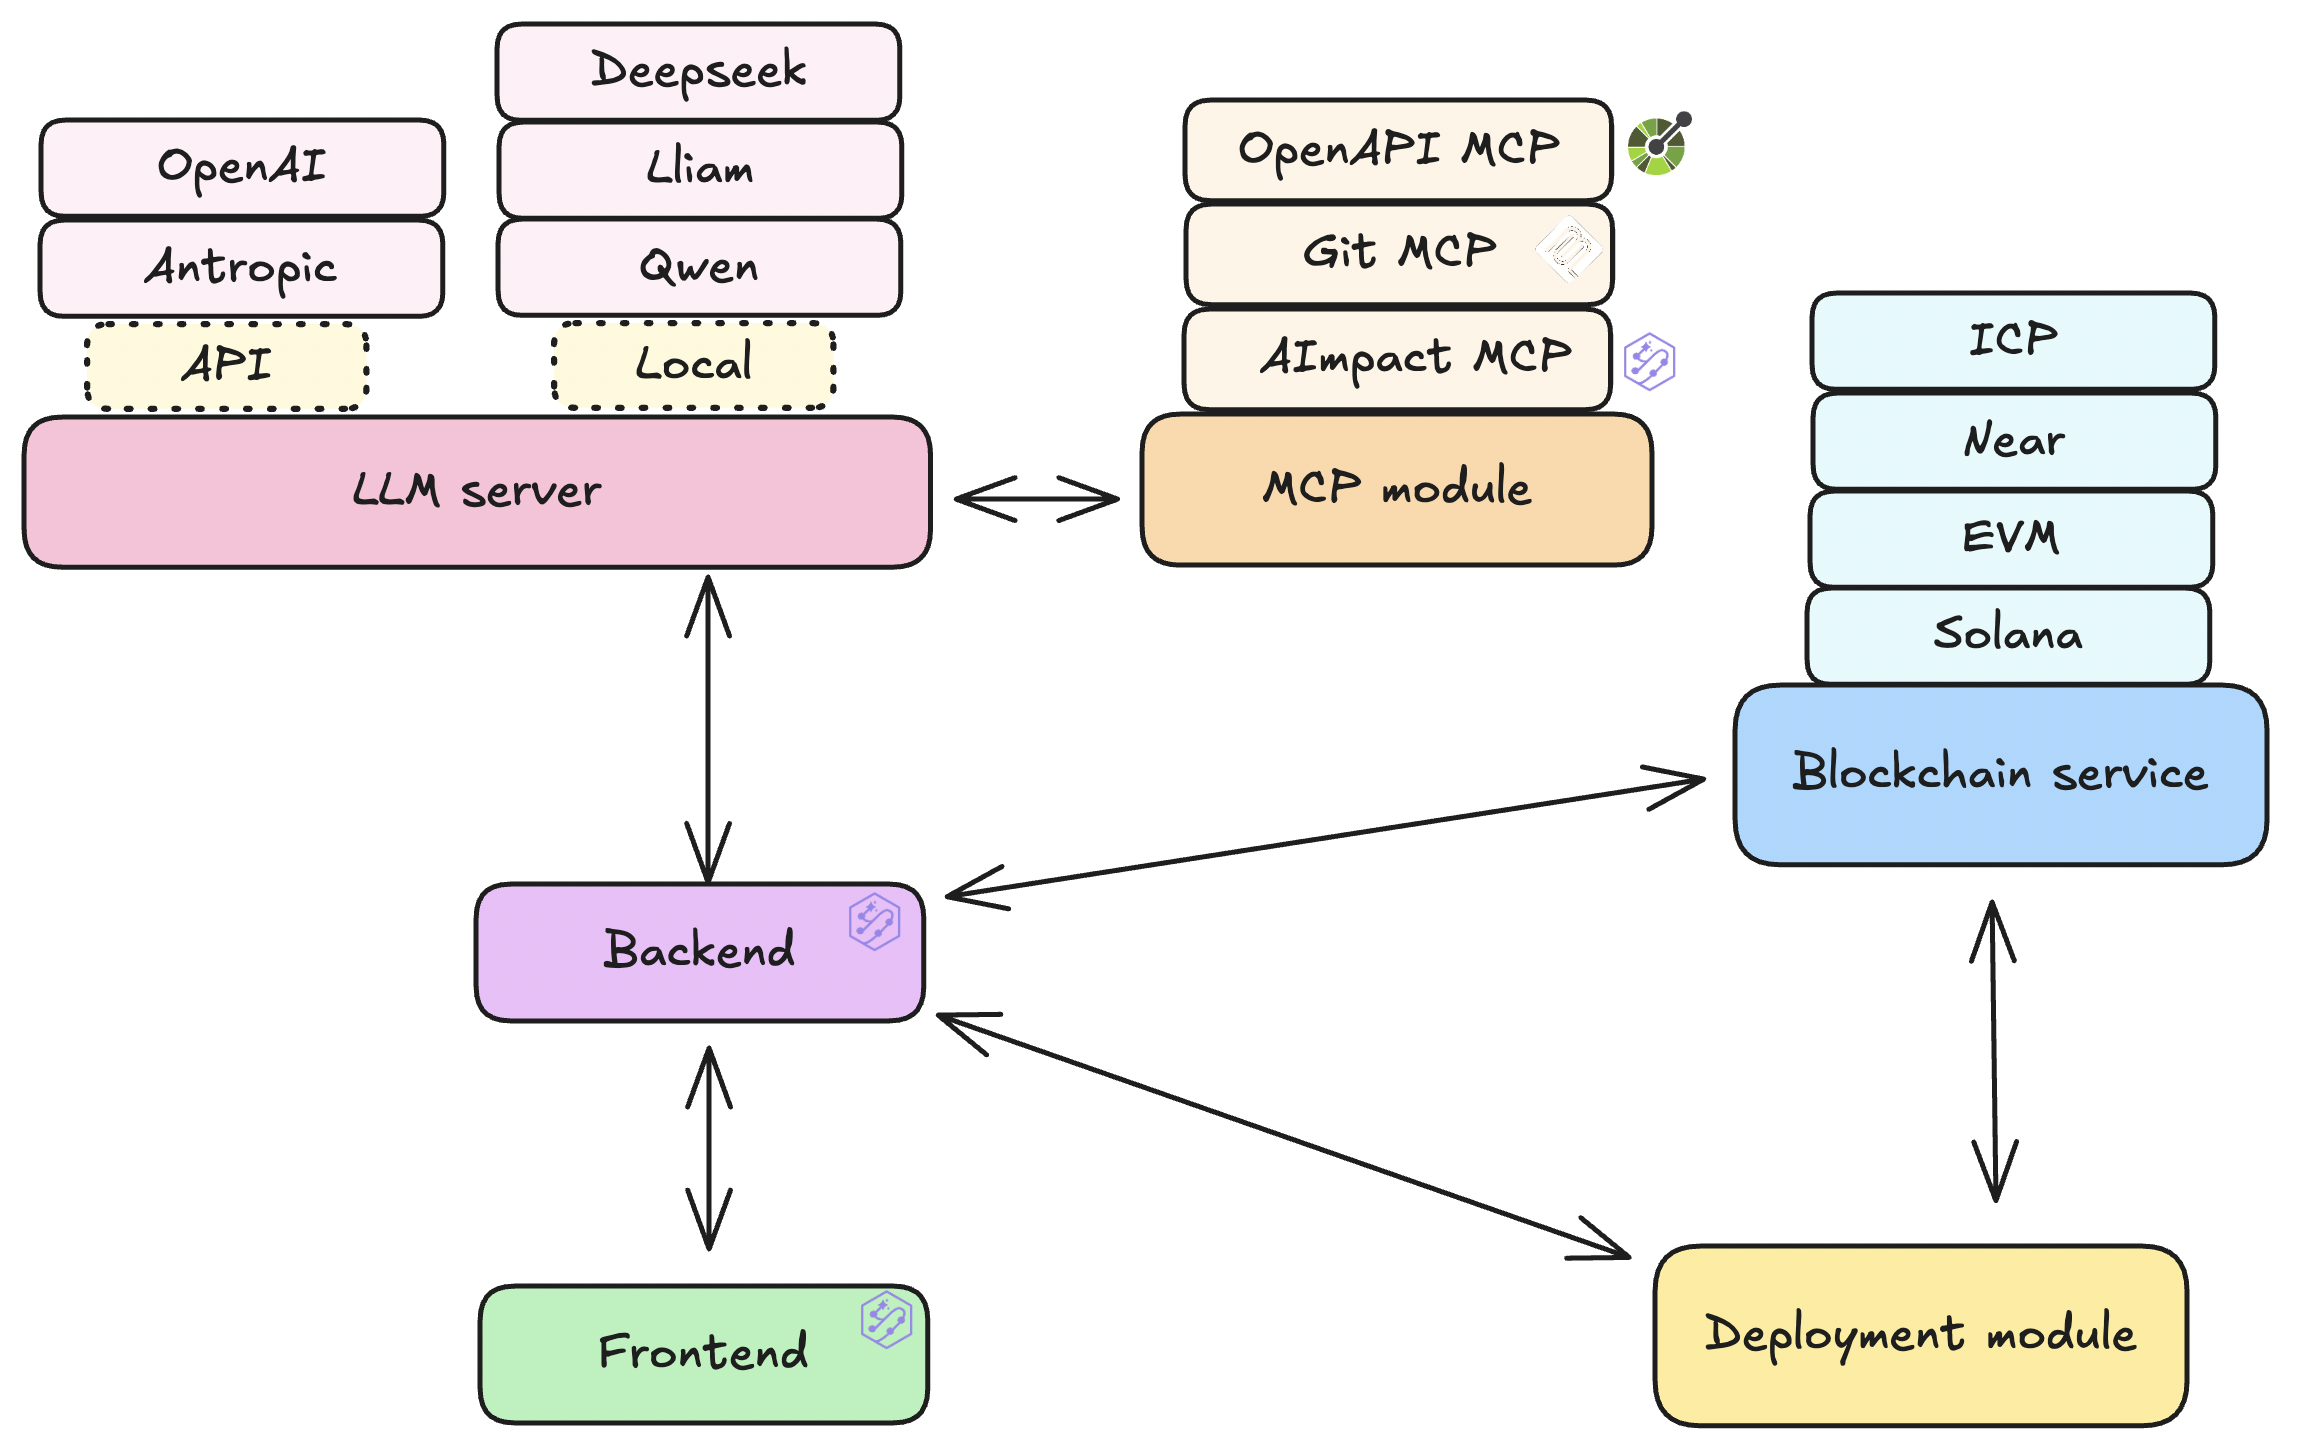
\includegraphics[width=0.7\textwidth]{imgs/architecture.png}
    \caption{Scheme of AImpact Infrastructure Architecture}
    \label{fig:architecture}
\end{figure}


\subsubsection{Frontend}

Frontend is the primary interface where users interact with the AImpact system. 
It provides an intuitive and user-friendly environment that abstracts the underlying complexity of blockchain technology and smart contract development. 
Through the frontend, users can describe their Web3 application requirements in natural language, monitor the development process, 
and manage their deployed applications.


\subsubsection{Backend}

The Backend serves as the central orchestration layer of the AImpact platform, coordinating communication between all system components. 
It handles user authentication, session management, and request routing to appropriate modules. 
Backend also manages the platform's database systems, storing user projects, smart contract templates, deployment configurations, and audit reports.


\subsubsection{MCP Module}

The Model Context Protocol (MCP) Module acts as the intermediary between the Large Language Model (LLM) and the platform's tools and resources. 
This module provides the LLM with structured access to smart contract templates, thirdparty APIs, blockchain deployment tools, and code analysis utilities. 

Components:
\begin{itemize}
    \item \textit{AImpact MCP}: Native MCP module.
    \item \textit{Thirdparty MCPs}:
        \begin{itemize}
            \item \textit{OpenAPI}: Provides access to public APIs on the internet.
            \item \textit{Git}: Manages git repositories.
        \end{itemize}
    .

\end{itemize}
\subsubsection{Blockchain Module}

The Blockchain Module manages blockchain-related operations within the AImpact platform. 
It provides abstracted interfaces for multiple blockchain networks. 
This module handles smart contract deployment, and interaction across different environments (testnet, devnet, and mainnet) 
as well as frontend deployment (ICP canister). 


\subsubsection{LLM Module}

The Large Language Model Module represents the core AI intelligence of the AImpact platform. 
It integrates multiple language models optimized for different tasks and using different resources. 

Models can be splitted into two groups:
\begin{itemize}
    \item \textit{Thirdparty based}: Proprietary models that are runned by thirdparty providers and accessed through API.
    \item \textit{Local based}: Open source models that are runned on the local machine and fine-tuned for the AImpact usecases.
\end{itemize}



\subsubsection{Deployment Module}

The Deployment Module manages the deployment for both smart contracts and frontend applications. 
For smart contracts, this module coordinates deployment across different blockchain networks, manages contract verification processes. 
For frontend applications, it integrates with the Internet Computer Protocol (ICP) for decentralized hosting, 
manages domain configurations, and ensures integration with deployed smart contracts. 
The module also implements deployment monitoring and automated health checks.


\subsection{Development Stages}

\subsubsection{Phase 1: Prototype development (MVP)}

\begin{itemize}
    \item No smart contract generation.
    \item Only single smart contract template.
    \item Frontend generation \& smart contract integration.
    \item Automated frontend deployment to centralised hosting provider.
\end{itemize}

This stage is used to test the platform and to get the market feedback.

\subsubsection{Phase 2: Smart contract generation}

\begin{itemize}
    \item Smart contract generation for single chain type (Solana, Ethereum, etc.).
    \item Smart contract templates for different use cases.
    \item Frontend generation \& smart contract integration.
    \item Smart contract deployment to all enviroments (sandbox, testnet, devnet, mainnet).
    \item Automated frontend deployment to the blockchain.
\end{itemize}

This stage presents a complete \textbf{basic} version of the product, which can be used by the users.


\subsubsection{Phase 3: MCP \& Multiple chains support }

\begin{itemize}
    \item AImpact MCP development \& support.
    \item Thirdparty MCPs support.
    \item Multiple chains support (Solana, Ethereum, Near, etc.).
    \item Smart contract templates for different use cases for different chains.
    \item Automated deployment of project components with MCP.
    \item Integrations with partners products.
\end{itemize}

This stage presents a complete version of the product with extended functionality.

% The userflow diagram in Figure \ref{fig:userflow} illustrates the end-to-end process of how users interact with the AImpact platform. Users begin by describing their desired Web3 application in natural language, which is then processed by our AI system to generate the appropriate smart contracts and frontend code. The platform handles all technical complexities, from contract deployment to frontend hosting, allowing users to focus solely on their application's core functionality and business logic.

\newpage

\begin{figure}[h]
    \centering
    \includegraphics[width=\textwidth]{imgs/tokenomics.png}
    \caption{AImpact Token Distribution and Utility}
    \label{fig:tokenomics}
\end{figure}









\end{document} 